%--Packages
\documentclass{article}
\usepackage[utf8]{inputenc}
\usepackage{fancyhdr} %--for fancy header/ footers
\usepackage{hyperref}
\usepackage{xcolor}
\usepackage{verbatimbox}
\usepackage{geometry}
\usepackage[pagestyles]{titlesec}
\usepackage{url}
\usepackage{graphics}


%--Parameters
\title{Proof of Concept I}
\author{Aaron Hammond\\43691455}
\date{September 2019}
\geometry{margin=2.5cm}
\fancyhfoffset{0em}
\definecolor{collink}{RGB}{45, 95, 140}
\titleformat{\section}{\normalfont\Large\bfseries}{}{0em}{}
\hypersetup{
colorlinks,
linkcolor=collink,
linktoc=all
}

%--Page Setup

\pagestyle{fancy}
\fancyhf{}

\rhead{Proof of Concept Design/ Deployment}
\lhead{Digital Humanities}

\fancyfoot[R,RO]{Aaron Hammond | 43691455}
\fancyfoot[L,LO]{Page: \thepage}

\renewcommand{\headrulewidth}{2pt}
\renewcommand{\footrulewidth}{1pt}
%--Commands

\newcommand\HRule{\rule{\textwidth}{1pt}} %-- horizontal lines for formatting

%--
\begin{document}

\begin{center}
%\HRule\\[0.4cm]
\huge{Proof of Concept Design/ Deployment}\\[0.4cm]
\huge{Aaron Hammond}\\[0.3cm]
\large{\today}\\[0.4cm]

\HRule \\[1cm]
\end{center}

%--

This document's purpose is to outline the software project that I have been working on for Digital Humanities. It is a solution that converts a range of file types to text files for analysis within the VoyantServer software. By placing the files in their necessary locations, this solution will convert and arrange all files within a directory ready for analysis and perform an export of the FIELDNOTES notebook in Joplin. Afterwards the user can simply open Voyant Server and select the converted and exported files for analysis.

\section{Prerequisites}
Please ensure that you are running Windows 10 and have the following software installed:
\begin{itemize}
    \item Ubuntu Distribution (available in the Windows Store)
    \item Java Version 8.0+
    \item Have 7zip installed (optional)
    
\end{itemize}

\section{Installation}
\subsection{Setup}
\begin{enumerate}
    \item In your C: create the folder FOAR705
    \item Download \href{http://docs.voyant-tools.org/resources/run-your-own/voyant-server/#download}{Voyant Server}
    \item Extract the zip file to C:/FOAR705
    \item Open the Ubuntu application
    \item Create a username and password
    \item Install the git package with the command sudo apt-get install git
\end{enumerate}

\subsection{Install Joplin}
\begin{enumerate}
    \item Install as per the instructions here https://joplinapp.org/
    \item Once installed, run joplin and login to your account
    \item Enter : to run commands
    \item Create a Notebook called FIELDNOTES
    \item Run the sync command by typing :sync
\end{enumerate}

\subsection{Install Deepspeech}
\begin{enumerate}
    \item Run command pip3 install deepspeech
\end{enumerate}


\subsection{Copy Repository Option: 1}
In Windows, Download and extract this file to the C:/FOAR705 folder

\url{https://cloudstor.aarnet.edu.au/plus/s/UPb7f1kUdGZMa7w}


\subsection{Copy Repository Option: 2}
If you prefer to copy the repository directly from Github - follow these instructions instead. This will copy the project repository, placing the relevant folder structure, scripts and necessary files onto your computer.
\vspace{0.5cm}
The folder structure should be as follows:\\
\vspace{0.5cm}
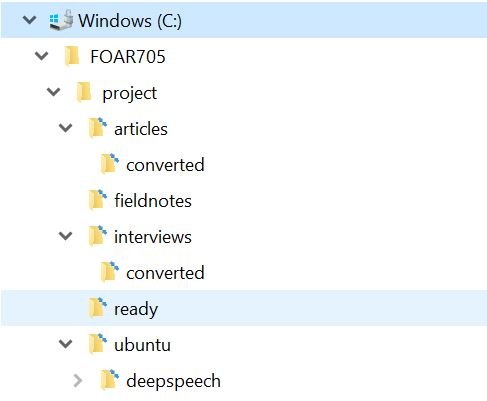
\includegraphics{folderstructure.JPG}

Navigate the Ubuntu terminal to your base C drive (cd /mnt/c/) and run the following commands:
\begin{enumerate}
    \item git clone https://github.com/MQ-FOAR705/HammondA\_PoC\_Design
    \item cd HammondA\_PoC\_Design
    \item mv project /mnt/c/foar705
    \item cd ..
    \item rm -r HammondA\_PoC\_Design
    \item cd /mnt/c/foar705/project/ubuntu/deepspeech
    \item curl -LO https://github.com/mozilla/DeepSpeech/releases/download/v0.5.1/deepspeech-0.5.1-models.tar.gz
    \item tar xvf deepspeech-0.5.1-models.tar.gz
    \item rm deepspeech-0.5.1-models.tar.gz
    \item mv deepspeech-0.5.1-models models
\end{enumerate}

\subsection{Placing the relevant files}
Within the project directory there is a set folder structure, interviews (for wav audio files), fieldnotes (for notes stored in Joplin) and articles (for PDF files). Currently there are test files already placed within these directories, if you would like to add your own please do so in the correct directory according to the file type.

\subsection{Scripts}
Open up the Ubuntu terminal, change directory to /mnt/c/foar705/ubuntu folder and bash the convertall script.

\subsection{Analysis}
\begin{enumerate}
    \item Open the Voyant Tools by running the VoyantServer.jar file within the previously extracted folder.
    \item Click Start Server
    \item Wait for web page to load
    \item Click the Upload button and navigate to the C:/FOAR705/Project/ready folder
    \item Select all files and click upload.
\end{enumerate}

\section{Stories and Acceptance Criteria}
\subsection{User Stories}
\begin{enumerate}
    \item As a researcher, I want the ability to convert PDF files into a simple text format.
    
    \item As a researcher, I want the ability to convert recorded conversations into a text format.
    
    \item As a researcher, I want to export my field notes for analysis.
    
    \item As a researcher, I want the ability to analyse various sources of data together.
    
    \item As a researcher, I want to organise my different sources so their origin can be easily identified.
    
    \item As a researcher, I want the ability to submit all my sources for analysis with a single step or upload.
    
    \item As a researcher, I want to be able to submit multiple files for conversion or upload in order to mitigate repeating tasks.
    
    \item As a researcher, I want the ability to analyse the lexicon of my source.
    
    \item As a researcher, I want to be able to identify and trace the analysis' results.
    
    \item As a researcher, I want the ability to access my data and research from other computers via. auto-backup to the cloud
    
\end{enumerate}

\section{Categorise user stories into themes and identify prerequisites}
The whole solution works according to three main steps. Conversion, Organisation and Analysis. This process depends on the file sources as already having been collected and available locally on my computer. Additionally the following steps must be performed in order from top to bottom. Items written in bold are steps that must be fulfilled to meet the requirements, items in italics are optional.
\subsection{Conversion}
This initial stage is concerned with converting the various types of sources into a single, workable format.

\subsubsection{Interviews}

As a researcher i should be able to:
\begin{enumerate}
    \item Store .wav files locally
    \item Transcribe them using Mozilla Deepspeech
    \item\textbf{Transcriptions are saved as simple-text files ready for analysis}
\end{enumerate}


\subsubsection{Literature}
As a researcher i should be able to:
\begin{enumerate}
    \item Select PDF documents for analysis
    \item Place them into a folder
    \item\textbf{Convert files into a simple-text files}
    \item\textbf{Files saved into a directory ready for analysis}
\end{enumerate}

\subsubsection{Fieldnotes}
As a researcher i should be able to:
\begin{enumerate}
    \item Run a command that syncs my Fieldnotes
    \item Export a preselected Notebook for analysis
    \item\textbf{Save filed notes into a folder for analysis}
\end{enumerate}

\subsection{Analysis}
As a researcher i should be able to:
\begin{enumerate}
    \item Open my preferred software for analysis
    \item\textbf{Import all converted sources for comparison analysis}
    \item\textit{View the results of the analysis and trace their origin}
    \item\textbf{Identify new links between sources}
    \item\textit{Export the results as a report for record keeping}
\end{enumerate}
\newpage
\section{Quality Assurance Testing}
\subsection{Ensure that deepspeech is installed correctly}
\begin{itemize}
    \item Open the Ubuntu terminal
    \item Type deepspeech
    \item Press enter
\end{itemize}
Receive the following response:
\begin{verbatim}
    usage: deepspeech [-h] --model MODEL --alphabet ALPHABET [--lm [LM]]
                  [--trie [TRIE]] --audio AUDIO [--version] [--extended]
deepspeech: error: the following arguments are required: --model, --alphabet, --audio
\end{verbatim}
\subsection{Convert audio files into text}
\begin{enumerate}
    \item Place audio files into the project/interviews folder
    \item Open the Ubuntu terminal
    \item Change directory to /mnt/c/FOAR705/project/ubuntu
    \item Bash script convertaudio.sh
    \item Check to ensure that the audio files are no longer in the interviews folder
    \item Check the interviews/converted folder to ensure the wav files have been moved there
    \item Check the project/ready folder to ensure that the transcription files files have been created
    \item Verify that the transcription files have the corresponding file name to the audio file's name and prefix of interview\_
    \item Open one of the interview\_ files in notepad to ensure its readability
\end{enumerate}
convertaudio.sh script contains the following:
\begin{verbatim}
    for f in /mnt/c/FOAR705/project/interviews/*.wav
do

deepspeech 
--model deepspeech/models/output_graph.pbmm 
--alphabet deepspeech/models/alphabet.txt 
--lm deepspeech/models/lm.binary 
--trie deepspeech/models/trie 
--audio $f > "${f%.wav}".txt;

mv $f /mnt/c/FOAR705/project/interviews/converted

done

cd /mnt/c/FOAR705/project/interviews

bash /mnt/c/FOAR705/project/interviews/rename.sh
\end{verbatim}
The rename.sh script contains the following
\begin{verbatim}
    for f in *.txt;
do
mv "$f" "interview_$f"
done

for renamed in *.txt
do
mv $renamed /mnt/c/FOAR705/project/ready
done

\end{verbatim}

\subsection{Convert PDF files into text}
\begin{itemize}
    \item Place PDF files for conversion into the project/articles folder
    \item Open the Ubuntu terminal
    \item Change directory to /mnt/c/FOAR705/project/ubuntu
    \item Bash script convertpdf.sh
    \item Check to ensure that the PDF files are no longer in the articles folder
    \item Check the articles/converted folder to ensure the PDF files have been moved there
    \item Check the project/ready folder to ensure that the text files files have been created
    \item Verify that the converted files have the corresponding file name to their original PDF file's name and prefix of article\_
    \item Open one of the article\_ files in notepad to ensure its readability
\end{itemize}
The convertpdf.sh script contains the following:
\begin{verbatim}
    for f in /mnt/c/foar705/project/articles/*.pdf
do
./pdftotext "$f" "$f.txt"

mv "$f" /mnt/c/foar705/project/articles/converted

done

cd /mnt/c/foar705/project/articles

bash renamemove.sh
\end{verbatim}
The renamemove.sh script contains the following:
\begin{verbatim}
for f in *.txt
do
mv "$f" "article_$f"

done

for f in *.txt
do
mv "$f" /mnt/c/foar705/project/ready
done

\end{verbatim}

\subsection{Ensure Joplin is installed and configured correctly}
\begin{itemize}
    \item Open the Ubuntu terminal
    \item Type joplin
    \item Press enter
    \item See the joplin application open and view your saved Notebooks and notes
    \item Type :sync
    \item Press enter
    \item See the status update and show the syncing process
    \item See the word Completed with the date and time of the sync
\end{itemize}

\subsubsection{Export FIELDNOTES notebook from Joplin and ready for analysis}
\begin{itemize}
    \item Open the Ubuntu terminal
    \item Change directory to /mnt/c/FOAR705/project/ubuntu
    \item Bash script convertnotes.sh
    \item Change directory to project/fieldnotes to ensure there is no files but the renameandmove.sh script
    \item Change directory to project/ready
    \item Verify that the notes from the FIELDNOTES notebook are present
    \item Check that each file has the prefix fieldnote\_
    \item Open one of the fieldnote text files to ensure it is uncorrupted
\end{itemize}

The convertnotes.sh script contains the following:
\begin{verbatim}
joplin sync
joplin export /mnt/c/foar705/project/fieldnotes/ 
--format md --notebook FIELDNOTES

for f in /mnt/c/foar705/project/fieldnotes/FIELDNOTES/*.md
do
mv "$f" /mnt/c/foar705/project/fieldnotes/

done

rmdir /mnt/c/foar705/project/fieldnotes/FIELDNOTES
rmdir /mnt/c/foar705/project/fieldnotes/_resources

cd /mnt/c/foar705/project/fieldnotes
bash renameandmove.sh

\end{verbatim}
The renameandmove.sh script contains the following:
\begin{verbatim}
    for f in *.md

do
mv "$f" "fieldnote_${f%.md}.txt"

done

for renamed in *.txt
do
mv "$renamed" /mnt/c/FOAR705/project/ready
done

\end{verbatim}

\subsection{Run all conversion scripts as a single step}
\begin{enumerate}
    \item Place 2 .wav files into the project/interviews folder
    \item Place 2 .pdf files into the project/articles folder
    \item Open the Ubuntu terminal
    \item Change directory to /mnt/c/FOAR705/project/ubuntu
    \item Bash the convertall.sh script
    \item Wait for the 'Everything converted successfully' message
    \item Navigate to the project/ready folder
    \item Ensure that there is a text file for each wav, pdf and note within the notebook
\end{enumerate}
The convertall.sh script contains the following:
\begin{verbatim}
bash convertpdf.sh
echo Finished converting PDF to text. Ready!
bash convertaudio.sh
echo Finished converting audio to text. Ready!
bash convertnote.sh
echo Finished exporting and converting notes. Ready!

echo Everything converted successfully!

\end{verbatim}

\subsection{Run Voyant Server for analysis}
\begin{enumerate}
    \item Open the VoyantServer folder
    \item Run the VoyantServer.jar file
    \item Click the 'Start Server' button and wait
    \item Once the webpage loads click the Upload button
    \item Navigate to the project/ready folder
    \item Select all files and click upload
    \item Look at the analysis and see that each file is easily identifiable due to its name and prefix 
\end{enumerate}


\end{document}
